Des travaux initiaux avaient été réalisés en Python par Samuel Charron. Il avait réalisé un plugin récupérant les signaux, construisant un classifier naïf bayésien multinomiale avec et permettant de classifier de nouveaux signaux. cependant les performances n'étaient pas suffisantes. N'étant pas formé au Python, j'ai préféré commencer mes travaux en utilisant le Java avec l'accord de Samuel. Je savais en m'orientant vers le Java, qu'une fois que l'application obtiendrait de bonnes performance, j'aurais à implémenter son fonctionnement général en Python sous forme de plugin.

\section{Démarche de travail}
    Ce projet s'inscrit parfaitement dans le type de projet R\&D. De ce fait, l'avancement est très difficile à planifier dans le temps. Surtout lorsque l'on ne connaît pas les différentes notions sous-jacentes au projet et qu'il y a une bonne part d'auto-formation avant de pouvoir développer une application.

    \subsection{Mes acquis à l'INSA}
        Les connaissances générales que j'avais en \textit{Data Science}, avant le début du stage, concernaient le \textit{Data Mining} en contexte \textbf{numérique} et étaient les suivantes :
        \begin{itemize}
            \item Concepts en analyse et normalisation de données : Analyse en Composantes Principales (ACP), centrage et réduction de données numériques ;
            \item Concepts d'apprentissage non-supervisé : méthodes de regroupement des données (Clustering : Classification Hiérarchique Ascendante, Algorithme des K-Means, Modèles de mélanges et Algorithmes EM) ;
            \item Base de l'optimisation : méthodes du gradient et de Newton, introduction aux outils mathématiques pour l'optimisation sous contraintes convexe ;
            \item Concepts d'apprentissage supervisé : méthodes pour la discrimination de données (Décision Bayésienne, Régression logistique, SVM linéaire) et notions de validation croisée.\\
        \end{itemize}

        Ce projet ne permet pas de mettre mes connaissances en apprentissage non-supervisé en avant. Cependant, mes notions d'apprentissage supervisé telles que : la démarche à suivre pour construire un classifieur, les concepts liées à la validation des performances (validation croisée) et la notion de sur-apprentissage ; ont été fort utiles.\\

        D'une manière générale, mes connaissances en \textit{Text Mining} n'étaient pas suffisamment étoffées pour pouvoir dire tel classifieur est plus performant qu'un autre dans tel contexte (binaire ou multi-classe). En effet, ma formation (à l'INSA) est axée manipulation et traitement de données en contexte \textbf{numérique}. De ce fait, la manipulation et le traitement de données textuelles m'étaient inconnus.\\

        Une formation en \textit{Text Mining} m'a donc été indispensable avant de pouvoir commencer à travailler.

    \subsection{Déroulement du stage}
        Ainsi, durant les deux premiers mois, j'ai exploré le domaine du \textit{Text Mining} et du \textit{Natural Language Processing} au travers de la bibliothèque de Stanford implémentée en Java (\textit{Stanford Natural Language Processing}). Conjointement, j'ai étudié les cours associés, et construit une première application Spring répondant aux contraintes évoquées en partie \ref{sec:ma_mission_chez_data_publica} (sauf le critère du langage). Le travail en ressortant est décrit en partie \ref{sec:travaux_realises_en_java}.\\

        Ensuite, lors du dernier mois, j’ai implémenté le comportement général de cette application sous la forme d’un plugin Python, visible en partie \ref{}. Certain composants n'existaient pas en Python, je les ai donc ré-implémenté.

\section{Travaux réalisés en Java, le \textit{Text Mining} et le \textit{Natural Language Processing} avec la bibliothèque de Stanford}
\label{sec:travaux_realises_en_java}
    \subsection{Présentation de mon environnement de travail}
        Dans C-Radar tout les traitements de type \og computing \fg (calcul) sont réalisés en Python (cf partie \ref{subsub:archi_tech}). De ce fait, créer une application permettant de classifier les signaux, devrait être fait en Python sous la forme d'un plugin (comme le requiert ma mission). Ayant fait le choix de commencer mes recherches en Java, il a fallu m'initialiser un environnement de travail un peu différent de l'environnement de travail Python.

        \paragraph{Spring et MongoDB :}
            Ainsi, Loïc Petit m'a créé une application Spring de base permettant de me connecter en local à une base de données Mongo. L'application me fournit un environnement de travail dans lequel construire le classifier à partir des signaux validés. Les signaux eux-mêmes récupérés depuis une base de données Mongo. Cette base de données contient mon ensemble de signaux permettant de construire et tester mon classifier. Les 1426 signaux validés y sont stocké ainsi que 350.000 autres signaux non validés (voir le dernier paragraphe de la partie \ref{sec:etat_bd}).\\

        Voici comment les signaux sont stockés dans Mongo :
\begin{verbatim}
{
    "id" : "TWITTER:agencenetdesign:329129810423083009",
    "content" : "Salon eCom Genève : l'équipe ND est en place au stand E1 \:) #ecomSITB http://t.co/YtsEs6rcDR",
    "publicationDate" : ISODate(2013-04-30T07:07:16Z),
    "sourceId" : "TWITTER:agencenetdesign",
    "source" : {
        "type" : "TWITTER",
        "resourceId" : "agencenetdesign"
    },
    "externalSignalId" : 329129810423083009,
    "validated" : false,
    "validatedTags" : [ ],
    "tags" : [
        "EVENT"
    ],
    "url" : "http://twitter.com/agencenetdesign/status/329129810423083009"
}
\end{verbatim}

        Le signal comporte :
        \begin{itemize}
            \item un identifieur unique \textit{id} ;
            \item un contenu \textit{content} ;
            \item une date de publication \textit{publicationDate} ;
            \item l'identifieur de la source \textit{sourceId} ;
            \item la source \textit{source} composé :
            \begin{itemize}
                \item du type de réseau dont provient le signal \textit{type} ;
                \item de l'identifieur du publieur dans ce réseau \textit{resourceId} ;
            \end{itemize}
            \item un identifeur externe \textit{externalSignalId} ;
            \item un booléen spécifiant si le signal a été manuellement validé ou non \textit{validated} ;
            \item la liste des tags s'il a été validé \textit{validatedTags}, la liste des tags potentiels (trouvés par le classifieur) \textit{tags} ;
            \item l'url là où a été publié le signal \textit{url}.
        \end{itemize}

        \paragraph{Formation Spring et Mongo :}
            Je me suis rapidement formé à Spring et Mongo pour pouvoir interfacer ces deux composants ensemble. Pour cela, j'ai suivi les tutoriels de Spring disponibles sur \href{https://spring.io/guides/gs/accessing-data-mongodb/}{https://spring.io/guides/gs/accessing-data-mongodb/}.\\
            Grâce aux tutoriels, j'ai appris à créer mes premiers points d'API permettant de faire des requêtes dans Mongo. Ces requêtes sont relativement basiques : récupérer tout les signaux sous forme de liste, récupérer uniquement les signaux validés (également sous forme de liste), savoir combien de signaux sont stockés dans ma base, etc. J'ai appris à faire ce type de requête dans Mongo grâce à la documentation sur \href{https://docs.mongodb.org/manual/}{https://docs.mongodb.org/manual/}. Les concepts de base de Mongo ne sont pas très compliqués à comprendre quand on a des notions de base de données.\\

        Dès que j'ai été capable de faire ce type de requêtes auprès de ma base de données, il fallait à présent me concentrer sur le traitement des signaux, et donc la construction du classifieur. C'est à ce moment que je me suis intéressé à la bibliothèque de Stanford.

        \subsection{La bibliothèque : Stanford Natural Language Processing}
            Samuel Charron avait connaissance de l'existence de cette bibliothèque. De ce fait, il m'a conseillé de me former en \textit{Text Mining} et en \textit{Natural Language Processing} au travers de celle-ci puisqu'elle est implémentée en Java. Je me suis donc plongé dedans afin de découvrir les diverses fonctionnalités qu'elle propose. Celle-ci propose un ensemble d'outils pour le traitement automatique du langage naturel de la langue anglaise, chinoise et espagnole. Voici ces différents outils.

            \subsubsection{Stanford POS Tagger (Part-Of-Speech) :}
                Le \textit{POS Tagger} permet de savoir la fonction grammaticale de chaque mot d'une phrase. Celui-ci fonctionne aussi pour le français.

                \paragraph{Exemple :}
                    Entrée \og Gustave is the firstname of a very famous french architect.\fg\\
                    Sortie :
\begin{lstlisting}
K$\overbrace{Gustave}^{\highlight[cyan]{NNP}} \overbrace{is}^{\highlight[green]{VBZ}} \overbrace{the}^{\highlight[magenta]{DT}} \overbrace{firstname}^{\highlight[cyan]{NN}} \overbrace{of}^{\highlight[orange]{IN}} \overbrace{a}^{\highlight[magenta]{DT}} \overbrace{very}^{\highlight[yellow]{RB}} \overbrace{famous}^{\highlight[yellow]{JJ}} \overbrace{french}^{\highlight[yellow]{JJ}} \overbrace{architect}^{\highlight[cyan]{NN}}\overbrace{.}^{\highlight[gray]{.}}$W
\end{lstlisting}
                \textit{$\highlight[cyan]{NNP}$} signifie qu'il s'agit d'un nom propre singulier (\textit{noun, proper, singular}), \textit{$\highlight[green]{VBZ}$} signifie qu'il s'agit d'un verbe à la 3ème personne du singulier au présent (\textit{verb, present tense, 3rd person singular}), \textit{$\highlight[magenta]{DT}$} signifie qu'il s'agit d'un déterminant (\textit{determiner}), \textit{$\highlight[cyan]{NN}$} signifie qu'il s'agit d'un nom commun singulier (\textit{noun, common, singular}), \textit{$\highlight[orange]{IN}$} signifie qu'il s'agit d'une préposition ou d'une conjonction de subordination (\textit{preposition or conjunction, subordinating}), \textit{$\highlight[yellow]{RB}$} signifie qu'il s'agit d'un adverbe (\textit{adverb}) et \textit{$\highlight[yellow]{JJ}$} signifie qu'il s'agit d'un adjectif (\textit{adjective}).

            \subsubsection{Stanford Parser :}
                Le \textit{Parser} permet de connaître la structure grammaticale d'une phrase, à savoir quel(s) groupe(s) de mots forme(nt) le sujet, quel(s) groupe(s) de mots forme(nt) le verbe et quel(s) groupe(s) de mots forme(nt) le complément. Cet outils est une sur-couche du \textit{POS Tagger}. En effet, il réutilise, entre autres, son résultat pour en déduire la structure grammaticale d'une phrase.

                \paragraph{Exemple :}
                Entrée \og My internship was a rewarding experience.\fg\\
                Sortie :
\begin{lstlisting}
K(\textcolor{blue}{ROOT}W
  K(\textcolor{blue}{S}W
    K(\textcolor{cyan}{NP} (\textcolor{pink}{PRP}\$ My) (\textcolor{cyan}{NN} internship))W
    K(\textcolor{green}{VP} (\textcolor{green}{VBD} was)W
      K(\textcolor{cyan}{NP} (\textcolor{magenta}{DT} a) (\textcolor{yellow}{JJ} rewarding) (\textcolor{cyan}{NN} experience))W
    K(\textcolor{gray}{.} .)))W
\end{lstlisting}
                Cet outils a pour vocation d'identifier les groupes de mots, ainsi que leurs dépendances à d'autres groupes de mots.

            \subsubsection{Stanford Named Entity Recognizer :}
                Le \textit{Named Entity Recognizer} permet d'identifier les groupes de mots qui sont des noms de personne, d'entreprises, de gènes, etc.

                \paragraph{Exemple :}
                Entrée \og François Bancilhon is the CEO of Data Publica, a Startup located in Paris.\fg\\
                Sortie :
\begin{lstlisting}
K$\highlight[magenta]{François}$W K$\highlight[magenta]{Bancilhon}$W is the CEO of K$\highlight[orange]{Data}$W K$\highlight[orange]{Publica}$W, a Startup located in K$\highlight[violet]{Paris}$W.
\end{lstlisting}
                Les mots surlignés en magenta comme $\highlight[magenta]{François}$ $\highlight[magenta]{Bancilhon}$ sont potentiellement des noms de personnes (\textit{$\highlight[magenta]{PERSON}$}). Ceux surlignés en orange comme $\highlight[orange]{Data}$ $\highlight[orange]{Publica}$ sont potentiellement des noms d'organisations (\textit{$\highlight[orange]{ORGANIZATION}$}). Enfin, les mots surlignés en violet comme $\highlight[violet]{Paris}$ sont potentiellement des noms de lieux (\textit{$\highlight[violet]{LOCATION}$}).

            \subsubsection{Stanford Classifier :}
                Le \textit{Classifier} permet de construire un classifieur automatique pour la catégorisation de texte. Un classifier est un outils d'apprentissage automatique qui prend des données et les classifie dans k classes. Un classifieur probabiliste peut aussi donner la distribution des probabilités de chaque classes pour une donnée. L’implémentation Java de Stanford est un classifieur \textit{maximum entropy}. Les modèles \textit{maximum entropy} sont aussi connu sous le noms de \textit{softmax classifiers} et sont équivalent aux modèles de régression logistique multi-classe (avec des paramètres différents, dans le sens où ce modèle est avantageux en cas de données sparse). Cet outils sera détaillé d'avantage par la suite.

            \subsubsection{Stanford CoreNLP :}
                Le \textit{CoreNLP} permet de construire une suite de traitements automatiques (les traitements précédents) sur de l'anglais, du chinois, de l'espagnol. Un exemple de chaîne de traitement est visible en figure \ref{fig:coreNLP}. La particularité de cet outils par rapport aux précédents, est qu'il permet de réutiliser les traitements précédents les uns à la suite des autres (sauf le \textit{Stanford Classifier}). De plus, il permet aussi d'appliquer des traitements supplémentaires à ceux énoncés jusque là. En effet, celui-ci réutilise certain des traitements précédents pour faire de la recherche morphologique telle que la lemmatisation ou du stemming. Le \textit{POS Tagger} et le \textit{Tokenizer} sont notamment réutilisés.

                %\paragraph{Fonctionnement :}
                %L'entité manipulée dans la classe \textit{StanfordCoreNLP} est le \textit{pipeline}. Le \textit{pipeline} est donc l'objet permettant de créer des chaînes de traitement. Il possède une liste de propriétés. Il suffit d'ajouter un objet appelé \textit{Annotator} aux propriétés du \textit{pipeline} pour que celui-ci réalise un traitement précis.\\
                %Par exemple, \textit{TokenizerAnnotator} est l'\textit{Annotator} permettant d'appliquer le traitement du \textit{Stanford Tokenizer} sur le texte donné en entrée.\\
                %Le fonctionnement est le suivant : Premièrement, il faut instancier un objet \textit{pipeline} et lui assigner des \textit{Annotators}. Ainsi, une série de traitements devra être réalisée lors de l'appel de sa méthode principale \textit{annotate()}. Ensuite, il n'y a plus qu'à passer une chaîne de caractère à cette méthode \textit{annotate()} pour obtenir un objet annoté en retour.

            \subsubsection{Lemmatisation :}
                La lemmatisation est le traitement consistant à trouver les lemmes de chaque mots d'une phrase. Ce traitement est détaillé en partie \ref{}. Pour cela, ce traitement nécessite que la phrase soit préalablement découpée en token (les mots de la phrase) et que chacun d'entre eux soit tagué par le \textit{POS Tagger}. Ainsi, en couplant la fonction grammaticale d'un mot avec un dictionnaire, il est possible de retrouver le lemme du mot.

                \paragraph{Exemple :}
                Entrée \og No better example than these could have been found.\fg\\
                Sortie :
\begin{lstlisting}
K$\overbrace{No}^{\highlight[yellow]{no}}\ \overbrace{better}^{\highlight[yellow]{good}}\ \overbrace{example}^{\highlight[cyan]{example}}\ \overbrace{than}^{\highlight[orange]{than}}\ \overbrace{these}^{\highlight[magenta]{this}}\ \overbrace{could}^{\highlight[green]{can}}\ \overbrace{have}^{\highlight[green]{have}}\ \overbrace{been}^{\highlight[green]{be}}\ \overbrace{found}^{\highlight[green]{find}} \overbrace{.}^{\highlight[gray]{.}}$W
\end{lstlisting}

            \subsubsection{Stemming :}
                Le stemming est un traitement assez similaire à la lemmatisation. En effet, celui-ci consiste à trouver les stems de chaque mots d'une phrase. Ce traitement est détaillé en partie \ref{}.

                \paragraph{Exemple :}
                Entrée \og Les chevaliers chevauchent leur chevaux, le cavalier son cheval.\fg\\
                Sortie :
\begin{lstlisting}
K$\overbrace{Les}^{le}\ \overbrace{chevaliers}^{cheva}\ \overbrace{chevauchent}^{cheva}\ \overbrace{leur}^{leur}\ \overbrace{chevaux}^{cheva} \overbrace{,}^{,}\ \overbrace{le}^{le}\ \overbrace{cavalier}^{caval}\ \overbrace{son}^{son}\ \overbrace{cheval}^{cheva} \overbrace{.}^{.}$W
\end{lstlisting}

            \begin{figure}[h!]
                \centering
                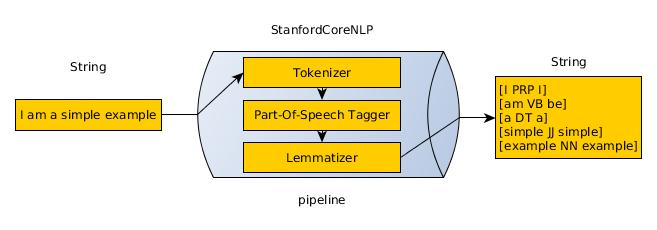
\includegraphics[width=\textwidth]{images/coreNLP.jpg}
                \caption{Trois traitements ont été assignés au \textit{pipeline} (entité de la classe \textit{StanfordCoreNLP}) : \textit{Tokenization}, \textit{POS-Tagging} et \textit{Lemmatization}. L'objet en sortie est une chaîne de caractère présentant le résultat de chaque traitement en colonne.}
                \label{fig:coreNLP}
            \end{figure}

            \subsubsection{Premier bilan sur la bibliothèque :}
                Ces traitements n'ont pas tous un intérêt pour moi dans la construction de mon classifieur. En effet, dans un premier temps, mon objectif est seulement de réutiliser la partie \textit{Stanford Classifier} de la bibliothèque pour créer un classifieur binaire permettant de classifier les signaux relatifs aux offres d'emploi et de stage (soit le tag \textit{JOB}).\\

                Cependant, il est certain que des traitement comme la lemmatisation ou le stemming me seront utiles par la suite, lorsqu'il faudra normaliser mes données.

        \subsection{Première mise en pratique de la bibliothèque de Stanford}
            \subsubsection{Ma première application Spring :}
                J'ai construis une application réalisant les actions suivantes (visible en figure \ref{fig:classif_building} et expliquée ci-après) :
            \begin{itemize}
                \item Récupérer les signaux stockés dans Mongo sous forme de liste ;
                \item Créer un ensemble de données à partir des signaux validés manuellement ;
                \item Diviser aléatoirement cet ensemble de données en deux ensembles (un pour entraîner le classifieur et un pour le tester) tout en gardant la proportion de chaque classe dans les deux ensembles ;
                \item Entraîner un classifieur binaire naïf bayésien ;
                \item Fixer les hyper-paramètres du classifier par validation croisée pendant la phase d'apprentissage ;
                \item Évaluer la qualité du classifieur construit (l'erreur de généralisation) en calculant sa précision et son rappel sur un ensemble de données de test (qui n'ont pas \og été vu \fg jusqu'à ici par le classifieur).
            \end{itemize}

            \begin{figure}[h!]
                \centering
                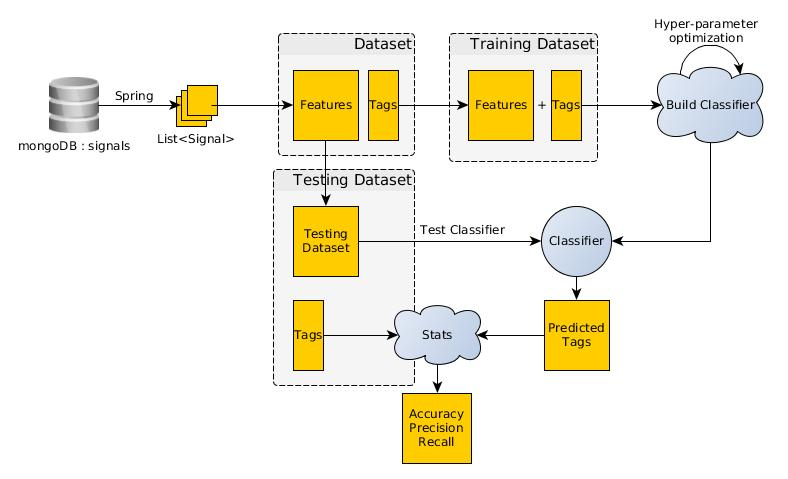
\includegraphics[width=\textwidth]{images/classifier_building.jpg}
                \caption{La construction du classifieur.}
                \label{fig:classif_building}
            \end{figure}

            \subsubsection{Le modèle de classifieur :}
                La première questions, à laquelle j'ai du répondre pour pouvoir créer un premier classifieur binaire sur la classe \textit{JOB}, est la suivante : Quel type de classifieur construire ? Un SVM, une régression logistique, une modèle naïf bayésien, etc.\\
                Dans la littérature de la classification de texte, comme la détection de spam dans les emails ou l'analyse des sentiments (savoir si un texte est critique ou élogieux), il est plutôt commun de construire des classifieurs naïf bayésien avec comme caractéristiques la fréquence des mots. Ainsi, j'ai choisi de construire un tel classifieur pour catégoriser mes signaux. (C'est également ce qu'avait fait Samuel Charron en Python.)

            \subsubsection{Construction de l'ensemble de données :}
                Ensuite, s'est poser la question de comment utiliser les données labellisées pour construire un ensemble de données pour l'apprentissage et la validation.\\
                Sur ce point, j'ai choisi de construire mon ensemble de données selon le modèle du sac de mots (\textit{bag of words}). Dans ce modèle, un texte (une phrase ou un document) est représenté comme un sac (\textit{bag}), un ensemble (au sens mathématique) de ses mots, sans se préoccuper de la grammaire ou de l'ordre des mots, mais en gardant la multiplicité. Ce modèle est communément utilisé en classification de document, quand la fréquence, l’occurrence des mots est utilisé comme caractéristique, attribut. Ce qui est le cas du modèle naïf bayésien. Ainsi, un signal est caractérisé par la liste des occurrences des mots formant son titre et son contenu.

            \paragraph{Exemple :}
                Voici deux signaux que l'on va modéliser à l'aide du sac de mots :
\begin{lstlisting}
K$Offre\ d'emploi\ :\ Ingénieur\ d’études\ et\ développement\ Java.$W
K$Offre\ de\ stage\ :\ Classification\ de\ signaux\ entreprises\ Java\ ou\ Python.$W
\end{lstlisting}
                À partir de ces deux signaux, une liste de mot est construite comme suit :
\begin{verbatim}
[ "Offre", "d'", "emploi", ":", "Ingénieur", "études", "et", "développement",
  "Java", ".", "de", "stage", "Classification", "signaux", "entreprises",
  "ou", "Python" ]
\end{verbatim}
                Celle-ci contient 17 mots distincts. En utilisant son index, on peut représenter chaque signal comme un vecteur de taille 17 :
\begin{lstlisting}
K$[\ 1,\ 2,\ 1,\ 1,\ 1,\ 1,\ 1,\ 1,\ 1,\ 1,\ 0,\ 0,\ 0,\ 0,\ 0,\ 0,\ 0\ ]$W
K$[\ 1,\ 0,\ 0,\ 1,\ 0,\ 0,\ 0,\ 0,\ 1,\ 1,\ 2,\ 1,\ 1,\ 1,\ 1,\ 1,\ 1\ ]$W
\end{lstlisting}
                Chaque ième composante du vecteur représente le nombre de fois que le ième mot de la liste est présent dans le signal. Par exemple, dans le premier vecteur (qui représente le premier signal), les deux premières composantes sont \og 1, 2 \fg. La première composante correspond au mot \og Offre \fg qui est le premier mot de la liste, et sa valeur est \og 1 \fg car \og Offre \fg est présent qu'une fois dans le premier signal. De la même façon, la deuxième composante correspond au mot \og d' \fg qui est le deuxième mot de la liste et sa valeur est \og 2 \fg car il est présent deux fois dans le signal. Cette représentation vectorielle ne préserve pas l'ordre des mots originel.\\

                Pour mon premier classifieur binaire naïf bayésien, l'ensemble de données a été construit suivant ce modèle, sur la base des 1426 signaux validés (présentés dans le dernier paragraphe de la partie \ref{sec:etat_bd}), en considérant seulement les 123 signaux validés \textit{JOB} comme intéressant.\\

                Enfin, aucun pré-traitement des données n'était mis en place, hors mis le fait de garder les mots dans le sac de mots final apparaissant un minimum de cinq fois. Ceci afin de supprimer les mots rares qui n'apportent pas d'informations lorsqu'on catégorise les signaux de type \textit{JOB} : les noms propres, les mots mal orthographiés ou les mots très spécifiques.

            \subsubsection{Construction du classifieur :}
                Une fois le problème de la construction de mon ensemble de données résolu, j'ai construis mon classifieur binaire naïf bayésien. Pour cela, j'ai divisé mon ensemble de données en deux ensemble de données dans les proportions suivantes :
                \begin{itemize}
                    \item 75\% de l'ensemble de données pour l'ensemble d'apprentissage ;
                    \item 25\% de l'ensemble de données pour l'ensemble de test.\\
                \end{itemize}
                À noter que la méthode de la bibliothèque, permettant de diviser l'ensemble de données en deux ensembles, ne garantis pas que la proportion des classes soit conservée dans les deux ensembles résultants. De plus, l'ensemble n'est pas mélangé à chaque nouvelle construction du classifieur, il y donc un risque de sur-apprentissage. Ces deux points, je ne les avais pas pris en compte directement car cela n'était pas explicitement expliqué dans la documentation de la bibliothèque. En effet, il a fallu que je m'aperçoive que les ensembles de données étaient toujours les mêmes en phase d'apprentissage et de test pour corriger ce point. Ainsi, j'ai du lire de plus près le code source de la méthode pour ré-implémenter le bon comportement.

            \subsubsection{Optimisation des hyper-paramètres par validation croisée :}
                Pour cette étape, une méthode de la bibliothèque se charge d'optimiser l'hyper-paramètre de mon classifieur naïf bayésien par validation croisée. Mon classifieur ayant été construit sur la base de l'ensemble d'apprentissage. Je l'ai donc utilisé sans aller plus loin dans les détails car la documentation n'en disait pas plus sur celui-ci et les performances en étaient bonifiées.

            \subsubsection{Évaluation de la qualité du classifieur :}
                Enfin pour évaluer l'erreur de généralisation de mon classifieur, je les testais sur un ensemble de test, que le classifieur n'avait pas \og vu \fg jusque ici. J'ai calculé la précision et le rappel obtenu par la classe \textit{JOB} et par la classe \textit{USELESS} représentant le reste n'appartenant pas à \textit{JOB}. Ceux-ci sont visible en table \ref{tab:classif_perf}.
                \begin{table}[h]
                    \centering
                    \begin{tabular}{| c | c | c |}
                        \hline
                         & \textit{JOB} & \textit{USELESS} \\
                        \hline
                        Précision & 0,84 & 0,99 \\
                        Rappel & 0,91 & 0,98 \\
                        \hline
                    \end{tabular}
                    \caption{Performances du classifieurs.}
                    \label{tab:classif_perf}
                \end{table}

            \subsubsection{Premier bilan :}
                Le classifieur construit est prometteur mais il ne s'agit que d'un classifieur binaire. La généralisation à plusieurs classes, va amener à faire de nouveau choix : Faut-il adopter une stratégie de type :
                \begin{itemize}
                    \item One versus all ;
                    \item One versus One.
                \end{itemize}
                D'autres questions peuvent être soulever comme :\\
                Est-ce que le modèle naïf bayésien va bien se généraliser en multi-classe ?\\
                Un prétraitement global n'est-il pas nécessaire ?\\
                Un prétraitement spécifique à chaque classe n'est-il pas nécessaire ?\\

        \subsection{Amélioration de ma première application et prétraitement}
            \subsubsection{Le passage au multi-classe :}
                Avant de pouvoir passer à un classifieur multi-classe
            \subsubsection{Les cours de l'université de Stanford :}
                Afin de perfectionner mon application, j'ai lu les cours de l’université de Stanford concernant le \textit{Natural Language Processing}, accessibles librement sur Internet. Ces cours proviennent du livre \textit{Introduction to Information Retrieval}\autocite{ir_web}.\\

                En parallèle, j'ai visionné sur coursera les vidéos que cette même université avait diffusé suite à un MOOC sur le \textit{Natural Language Processing}. Grâce à ces cours, j'ai pris conscience de toute l'importance du travail de prétraitement nécessaire à mettre en place, afin de bien normaliser et formater les données textuelles avant d'en faire quelque chose.\\

                Cette remarque prend tout son sens quand les données manipulées en plus d'être textuelles, ne sont pas normalisées (ou pas structurées).\\

                Durant ma formation au \textit{Natural Language Processing}, j'ai également lu les livres \textit{Natural Language Processing with Python}\autocite{nlp_p} et \textit{Python 3 Text Processing with NLTK 3 Cookbook}\autocite{nltk} , ainsi que les pages internets \textit{Introduction to Information Retrieval}\autocite{ir_web}.

            \subsection{Les travaux de prétraitement :}



            \paragraph{Le QA ou Quality Assessment :}
                L'objectif du QA est de demander la contribution d'un maximum de personnes sur une tâche de validation manuelle pénible.\\
                Durant mon stage j'ai organisé plusieurs QA pour approfondir l'ensemble des signaux d’apprentissage et de test.

La proportion des classes de cet échantillon est mauvaise, c'est-à-dire que les données souffrent d'un fort déséquilibre entre classes : il y a beaucoup plus de signaux inintéressants qu'intéressants. Je n'avait donc pas assez d'exemples de signaux intéressants pour pouvoir considérer les éventuelles prédictions d'un classifieur construit sur la base de ces données comme correctes. Il est donc nécessaire d'en valider d'autres manuellement.

            \paragraph{Proportion de signaux intéressants :}
                La quantité de signaux n'ayant pas d'intérêt, ici, est énorme (plus de 70\%). De ce fait, une pré-sélection des signaux à valider est nécessaire.\\
                Ainsi, j'ai réutilisé le premier classifieur implémenté en Python, construit sur la base des 1426 signaux. Ce classifieur a permis de classifier des signaux non validés.\\
                Ce sont ces signaux classifiés par le classifieur Python qui ont été sélectionnés pour être validés manuellement. Notamment ceux appartenant aux catégories EVENT, JOB et PRODUCT.\\
                Pour ceux appartenant aux catégories MONEY et PEOPLE, ils ont été sélectionnés pour être validés à l'aide d'expressions rationnelles pour faire ressortir des termes tels que \og levée de fonds \fg, \og chiffre d'affaire \fg, \og nommer \fg, \og nomination \fg, etc.
                De cette manière 2574 nouveaux signaux ont été validés manuellement.\\



            Au 27.07.2015, il y avait donc 4000 signaux validés manuellement par un humain :
            \begin{itemize}
                \item 488 catégorisés EVENT soit 12,2\%
                \item 258 catégorisés JOB soit 6,4\%
                \item 118 catégorisés MONEY soit 3\%
                \item 83 catégorisés PRODUCT soit 2,1\%
                \item 49 catégorisés PEOPLE soit 1,3\%
                \item 3004 validés mais considérés comme inintéressant soit 75\%
            \end{itemize}
